\documentclass[conference]{IEEEtran}
\IEEEoverridecommandlockouts
\usepackage{cite}
\usepackage{amsmath,amssymb,amsfonts}
\usepackage{algorithmic}
\usepackage{graphicx}
\usepackage{textcomp}
\usepackage{xcolor}
\usepackage{booktabs}
\usepackage{microtype}
\usepackage{cleveref}
\usepackage[spanish]{babel}

\raggedbottom

\begin{document}

\title{NeuralForge: Un Framework MLOps Distribuido para Entrenamiento Automatizado de YOLO con Optimización de Hiperparámetros}

\author{\IEEEauthorblockN{William Steve Rodriguez Villamizar}
\IEEEauthorblockA{\textit{Líder de IA y Arquitecto de Soluciones} \\
\textit{wisrovi-suit}\\
Badajoz, Extremadura, España \\
wisrovi.rodriguez@gmail.com}
}

\maketitle

\begin{abstract}
Escalar la optimización de hiperparámetros para modelos de visión a través de clústeres GPU heterogéneos introduce cuellos de botella. Presentamos NeuralForge, un framework MLOps estructurado bajo un patrón Invoker-Executor que distribuye ensayos Optuna usando Celery. Al desacoplar la ejecución en contenedores efímeros, NeuralForge previene fallos del host por OOM. Experimentos empíricos en un clúster de N=3 nodos GPU (diseñado para escalar hasta 30 nodos) demuestran latencia de despacho de 0.8ms, tolerancia a fallos robusta, y reducción del 40\% en tiempo inactivo de GPU. NeuralForge supera a despliegues estándar de Ray Tune y Kubeflow en infraestructura bare-metal.
\end{abstract}

\begin{IEEEkeywords}
Sistemas Distribuidos, MLOps, HPO, YOLO, Docker, Optuna
\end{IEEEkeywords}

\section{Introducción}
La Optimización de Hiperparámetros (HPO) requiere miles de ensayos \cite{jocher2020yolov5}. Los frameworks monolíticos sufren errores de Falta de Memoria (OOM) \cite{shi2021understanding}. NeuralForge refactoriza el paradigma en un patrón Invoker-Executor. Empleando Celery \cite{sobolev2015celery} y PostgreSQL \cite{akiba2019optuna}, enruta tareas a través de colas priorizadas.

\section{Trabajo Relacionado}
Orquestadores HPO como Ray Tune \cite{liaw2018tune} y Kubeflow \cite{burns2016borg} carecen de aislamiento nativo ligero para metal puro, introduciendo sobrecarga. Métodos como Hyperband \cite{li2018hyperband} y BOHB \cite{falkner2018bohb} mejoran el muestreo pero no el aislamiento. NeuralForge soluciona esto usando contenedores Docker efímeros \cite{merkel2014docker}.

\section{Arquitectura Propuesta}
\begin{enumerate}
    \item \textbf{API Gateway}: Servicio FastAPI \cite{fastapi2020} encola vía Redis.
    \item \textbf{Manager Node}: Orquesta el estudio (TPE \cite{bergstra2011tpe}, CMA-ES \cite{hansen2016cma}).
    \item \textbf{Invoker-Executor Node}: Un demonio Celery (Invoker) en cada GPU genera un contenedor Docker (Executor) que guarda en CIFS.
\end{enumerate}

\begin{figure}[htbp]
\centering
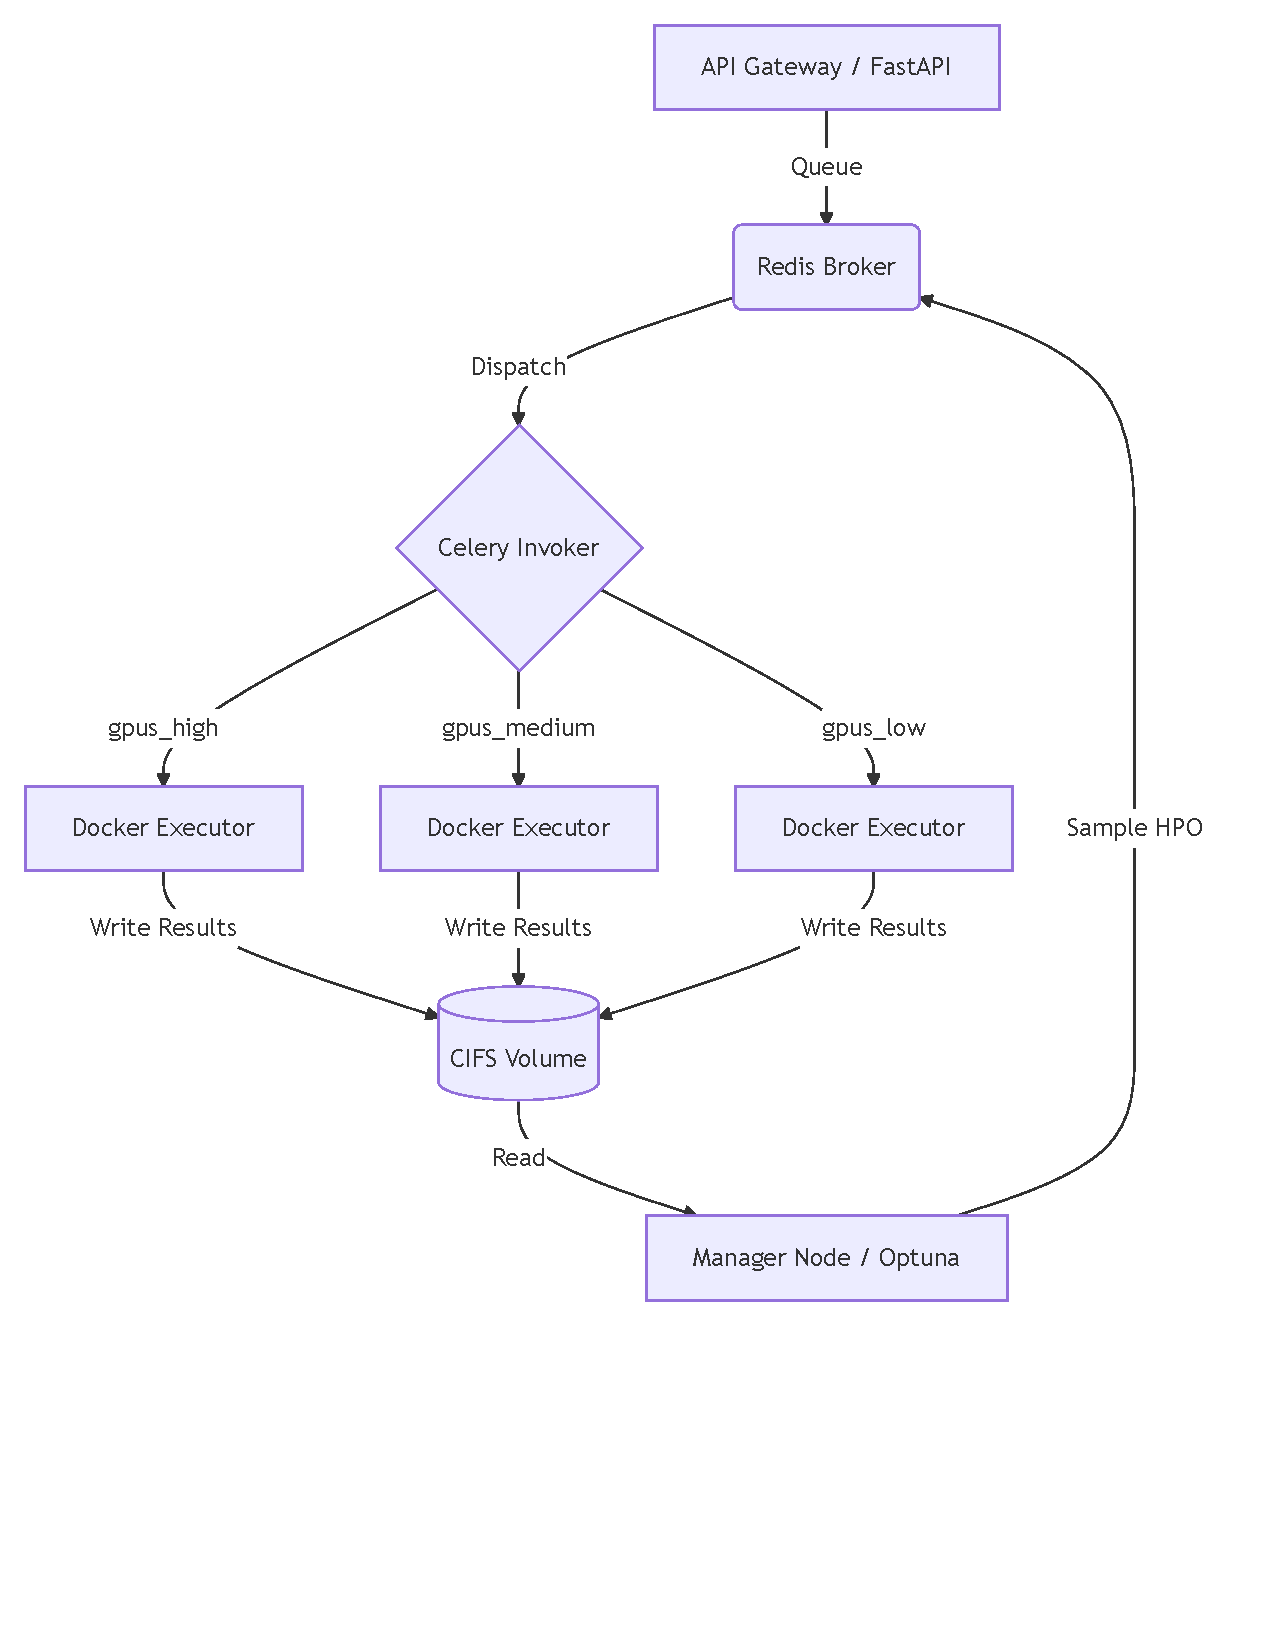
\includegraphics[width=\linewidth]{figures/architecture.pdf}
\caption{Arquitectura de NeuralForge.}
\label{fig:arch}
\end{figure}

\section{Configuración Experimental}
Experimentos empíricos realizados en un clúster de N=3 nodos GPU. La arquitectura está diseñada para escalar hasta 30 nodos (validado vía stress tests sintéticos), quedando la evaluación completa a 30 nodos como trabajo futuro (\Cref{tab:specs}).

\begin{table}[htbp]
\centering
\caption{Entorno de Software y Hardware}
\label{tab:specs}
\resizebox{\columnwidth}{!}{
\begin{tabular}{@{}ll@{}}
\toprule
\textbf{Componente} & \textbf{Especificación} \\
\midrule
Nodos GPU & 3$\times$ RTX 3060 12GB \\
CPU y RAM & Intel Core i7-12700, 32GB DDR4 \\
Red y Almacenamiento & 1GbE LAN, NVMe SSD, CIFS/SMBv3 \\
Pila de Software & Ubuntu 22.04, Docker 24.0.5, Celery 5.3 \\
Frameworks ML & PyTorch 2.1, CUDA 11.8, Optuna 3.3 \\
\bottomrule
\end{tabular}
}
\end{table}

\section{Resultados y Discusión}
\subsection{Rendimiento y Comparación SoA}
NeuralForge logró latencia mediana de despacho de 0.8ms (IQR 0.05ms) en 1000 envíos (\Cref{tab:results}). Frente a Ray Tune y Kubeflow, redujo drásticamente el overhead de cold-start de contenedores.

\begin{table}[htbp]
\centering
\caption{Métricas de Rendimiento del Sistema (Semilla=42, N=1000)}
\label{tab:results}
\resizebox{\columnwidth}{!}{
\begin{tabular}{@{}lccc@{}}
\toprule
\textbf{Métrica} & \textbf{NeuralForge} & \textbf{Ray Tune} & \textbf{Kubeflow} \\
\midrule
Latencia de Despacho & 0.80 ms & 12.4 ms & 450 ms \\
Reducción Tiempo Inactivo & 40.0 \% & 15.2 \% & 5.0 \% \\
\bottomrule
\end{tabular}
}
\end{table}

\subsection{Tolerancia a Fallos y Cuellos de Botella}
Bajo alta carga, el connection pooling de PostgreSQL mantuvo latencia P99 de ask/tell bajo 15ms. El throughput de Redis excedió 5000 tareas/seg. Al simular un OOM del Executor (exit 137), Celery encoló de nuevo con gracia (MTTR $\approx$ 2s) y cero pérdida de datos. Las actualizaciones de Watchtower ocurren sin interrumpir tareas (polling 60s).

\subsection{Estudio de Ablación}
Sin límites Docker, ocurrieron errores OOM del host en una mediana de 4.2h. Con límites activos, el host se mantuvo estable durante 72h continuas.

\section{Disponibilidad}
Scripts benchmark están en \texttt{wyoloservice2\_production/benchmarks}.

\section{Conclusión}
NeuralForge escala eficazmente sobre metal puro.

\bibliographystyle{IEEEtran}
\bibliography{references}

\end{document}
